
\begin{frame}{Resultados}
	Teste de latência para leituras
	\begin{columns}
		
		\column{0.5\textwidth}
		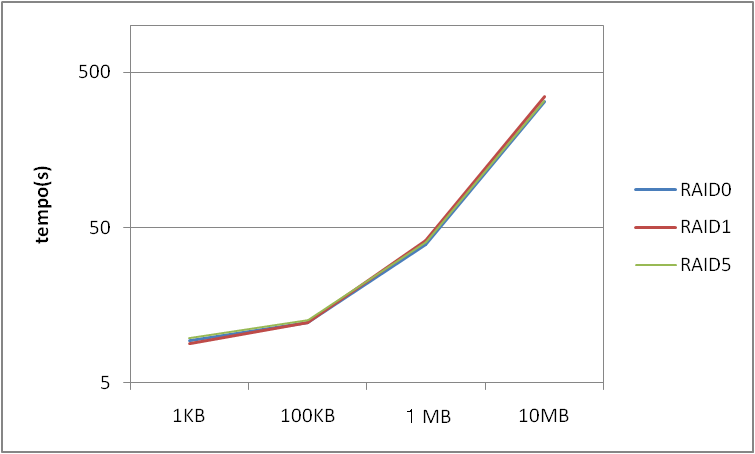
\includegraphics[width=\textwidth]{imagens/latencia_leitura}
		
		
		\column{0.5\textwidth}
	
		\begin{table}
			\caption{Tabela de valores(s)}
			\tiny
			\begin{tabular}{|c|c|c|c|c|} \hline
				& 1KB  & 100KB & 1MB   & 10MB  \\ \hline
				RAID 0	& 9.33 & 12.26 & 38.84 & 324.73\\ \hline
				RAID 1	& 9.01 & 12.19 & 41.50 & 348.15\\ \hline
				RAID 5	& 9.76 & 12.62 & 40.11 & 326.75\\ \hline
				
				
			\end{tabular}
		\end{table}
			
		
		
	\end{columns}
	%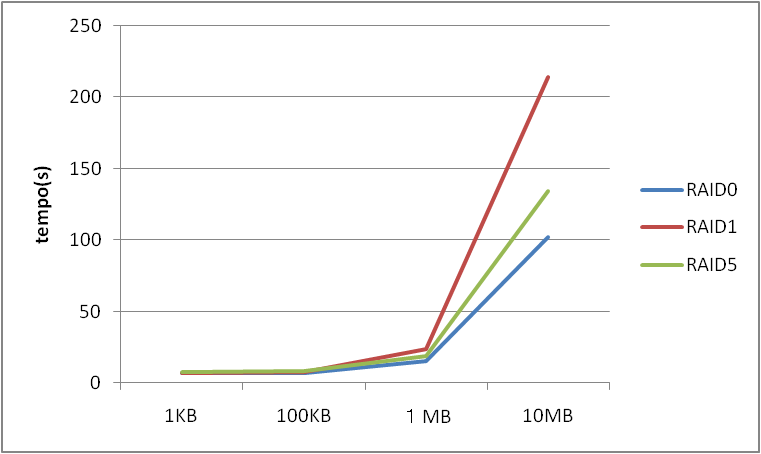
\includegraphics[width=0.5\textwidth]{imagens/latencia_escrita}
\end{frame}

\begin{frame}{}
	Teste de latência para escritas
	\begin{columns}
		
		\column{0.5\textwidth}
		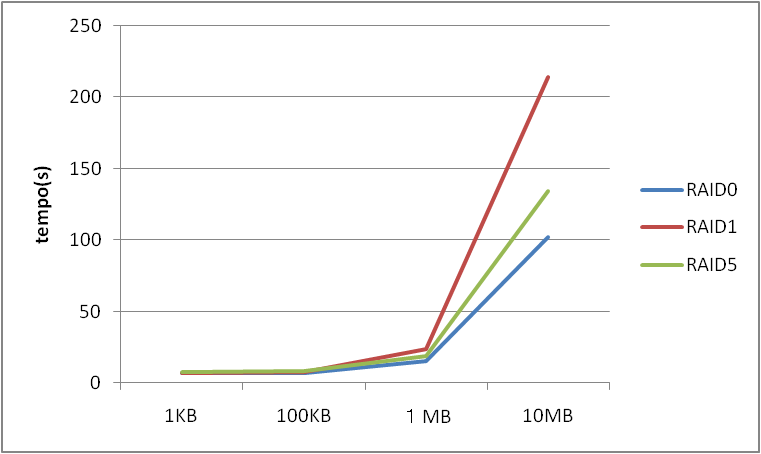
\includegraphics[width=\textwidth]{imagens/latencia_escrita}
		
		
		\column{0.5\textwidth}
		\begin{table}
			\caption{Tabela de valores(s)}
			\tiny
			\begin{tabular}{|c|c|c|c|c|} \hline
				& 1KB  & 100KB & 1MB   & 10MB \\ \hline
				RAID 0	& 6.70 & 6.91 & 14.92 & 101.93\\ \hline
				RAID 1	& 6.79 & 7.53 & 23.79 & 213.94\\ \hline
				RAID 5	& 7.31 & 7.91 & 18.26 & 134.31\\ \hline
				
				
			\end{tabular}
		\end{table}
		
	\end{columns}
\end{frame}


\begin{frame}{}
	Teste de vazão para leituras
	\begin{columns}
		
		\column{0.5\textwidth}
		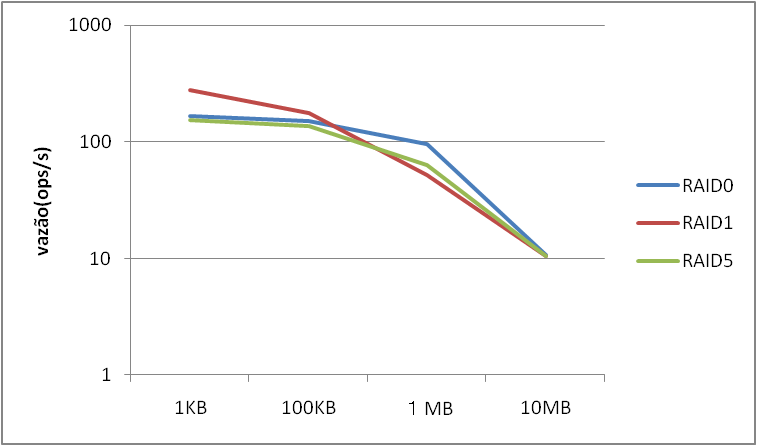
\includegraphics[width=\textwidth]{imagens/throughput_leitura}
		
		
		\column{0.5\textwidth}
		\begin{table}
			\caption{Tabela de valores(ops/s)}
			\tiny
			\begin{tabular}{|c|c|c|c|c|} \hline
				& 1KB & 100KB & 1MB & 10MB \\ \hline
				RAID 0	& 167.14 & 151.63 & 95.08 & 10.63\\ \hline
				RAID 1	& 278.86 & 177.43 & 51.92 & 10.52\\ \hline
				RAID 5	& 152.79 & 135.30 & 63.34 & 10.56\\ \hline
				
				
			\end{tabular}
		\end{table}
		
	\end{columns}
\end{frame}


\begin{frame}{}
	Teste de vazão para escritas
	\begin{columns}
		
		\column{0.5\textwidth}
		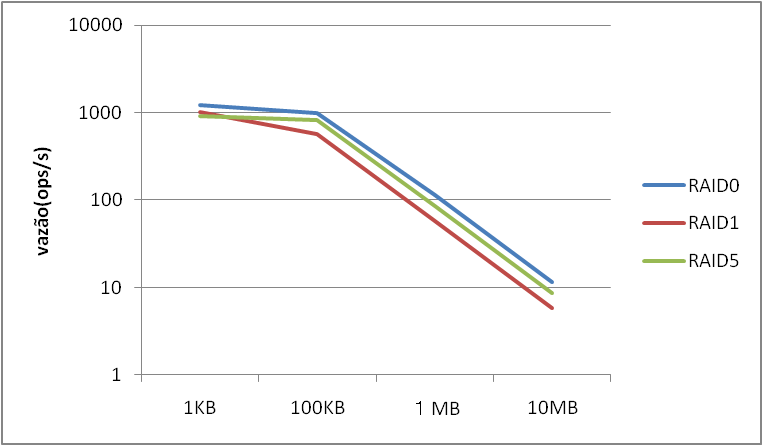
\includegraphics[width=\textwidth]{imagens/throughput_escrita}
		
		
		\column{0.5\textwidth}
		\begin{table}
			\caption{Tabela de valores(ops/s)}
			\tiny
			\begin{tabular}{|c|c|c|c|c|} \hline
				& 1KB & 100KB & 1MB & 10MB \\ \hline
				
				RAID 0	& 1209.19 & 988.14 & 113.07 & 11.51\\ \hline
				RAID 1	& 1023.54 & 571.43 & 58.01  & 5.76 \\ \hline
				RAID 5	& 914.91  & 830.56 & 84.52  & 8.66 \\ \hline
				
				
			\end{tabular}
		\end{table}
		
	\end{columns}
\end{frame}

